% =====================================================================
\chapter{KIỂM THỬ VÀ ĐÁNH GIÁ HỆ THỐNG}\label{chap:kiemthu}
% =====================================================================

Chương này trình bày chiến lược và kết quả kiểm thử (tự động, tích hợp bằng công cụ giả lập
và trên phần cứng), kết quả thực nghiệm trên mô hình, từ đó đánh giá các chức năng đã hoàn
thiện, các hạn chế đã khắc phục và các hạn chế còn tồn tại cùng nguyên nhân và cách khắc phục.


\section{Chiến lược kiểm thử}
\begin{figure}[H]
\centering
\begin{tikzpicture}[
  lv/.style={draw,rounded corners=2pt,font=\footnotesize,align=center,text width=4.5cm,minimum height=2.1cm},
  arr/.style={-{Stealth[length=2.5mm]},draw=black!70}]
\node[lv,fill=boxB] (a) at (0,0) {\textbf{Kiểm thử tự động trên máy tính}\\module máy chủ + mã nguồn hai client · 429 phép kiểm tra · vài giây};
\node[lv,fill=boxC] (b) at (5.5,0) {\textbf{Kiểm thử tích hợp bằng công cụ giả lập Python}\\\texttt{udp\_sender.py} · \texttt{udp\_rfid\_sender.py}};
\node[lv,fill=boxD] (c) at (11,0) {\textbf{Kiểm thử hệ thống trên phần cứng}\\30 kịch bản S1–S30};
\draw[arr] (a) -- (b); \draw[arr] (b) -- (c);
\end{tikzpicture}
\caption{Ba tầng kiểm thử: càng xuống dưới càng nhanh, tự động và chạy thường xuyên}\label{fig:testpyramid}
\end{figure}

\section{Kiểm thử tự động}
Bộ kiểm thử nằm trong \file{tests/} và chạy bằng \code{make -C tests}. Các module
nghiệp vụ của máy chủ được biên dịch với hai header giả (critical section và đồng hồ
điều khiển được). Hai sketch Arduino được biên dịch \emph{nguyên vẹn} cùng lớp giả lập
thư viện (\file{tests/arduino/}): đồng hồ \code{millis()}, mức logic từng chân, ADC,
Wi-Fi, UDP, đầu đọc MFRC522 và DHT11.

\begin{table}[H]
\centering\footnotesize
\caption{Các bộ kiểm thử tự động và kết quả}\label{tab:unittests}
\begin{tabularx}{\linewidth}{@{}lXr@{}}
\toprule
\textbf{Bộ} & \textbf{Nội dung kiểm tra} & \textbf{Kết quả} \\ \midrule
\file{payment} & CRC16-CCITT với giá trị kiểm tra chuẩn \code{0x29B1}; chuỗi VietQR đúng từng trường (00, 01, 38, 53, 54, 58, 62, 63); trùng từng byte với mã VietQR mẫu đã công bố (\code{\ldots{}6304AB76}); từ chối BIN sai, tài khoản trống hoặc có ký tự lạ, số tiền 0, nội dung có khoảng trắng, bộ đệm quá nhỏ; tìm giao dịch SePay theo mã (kể cả mã viết thường), chỉ chấp nhận đúng số tiền, từ chối trả dư, trả thiếu và mã khác; đọc id giao dịch mới nhất & 38/38 \\
\file{json\_parsers} & Bản tin hợp lệ (mọi thứ tự khóa, khoảng trắng, giới hạn dải); 22 bản tin \code{parking\_update} sai và 16 bản tin \code{rfid\_event} sai đều bị từ chối (thiếu/thừa khóa, khóa lặp, sai kiểu, ngoài dải, ký tự lạ, dữ liệu thừa, chuỗi có ký tự thoát); bản tin \code{climate} hợp lệ và 8 dạng sai; trường \code{seq} của \code{rfid\_event}: thiếu, bằng 0, âm, thập phân, số mũ, dạng chuỗi, vượt 32 bit, lặp khóa đều bị từ chối, giá trị $2^{32}-1$ đọc chính xác & 78/78 \\
\file{rfid\_session} & Phí theo giờ (biên 0, 3600, 3601\,s, bão hòa); vào/ra, sai cổng; hóa đơn hết hạn đúng 60\,s; bãi đầy, tái sử dụng chỗ; nhiệt độ; nhật ký vòng (thứ tự, chỉ giữ 10); thông báo từ chối 5\,s; IR báo đủ 5 ô thì từ chối thẻ mới; lưu rồi khôi phục sau ``mất điện'' (phiên, nhật ký, các \code{seq} đã xử lý, đồng hồ); đặt giờ Unix dời đúng các mốc cũ, lần đặt thứ hai không dời lại; chỉ mốc sau khởi động bị dời khi bù thời gian mất điện; bản lưu hỏng bị bỏ qua; cảm biến im lặng quá 3\,s thành ngoại tuyến và dữ liệu cũ không chặn xe vào; cảnh báo ngập bật ở 20\,mm, tắt ở 15\,mm, chặn xe vào nhưng vẫn cho ra; doanh thu và lượt vào/ra theo ngày, sang ngày mới, ra khỏi cửa sổ 7 ngày; \code{seq} gửi lại chỉ được xử lý một lần, nhớ 16 giá trị gần nhất; thanh toán QR: quẹt ra thành chờ thanh toán, quẹt lại hiện cùng mã QR, xe khác bị báo bận, sai mã không hoàn tất, trả xong thì có hóa đơn, nhật ký \code{OUT} và doanh thu, không ra hai lần, hết 180\,s có thông báo, chuyển khoản muộn vẫn được nhận, xác nhận tiền mặt cho xe đang chờ và xe chưa quẹt ra, tắt thanh toán thì ra ngay như cũ; xóa xe: rời danh sách, hủy lượt thanh toán và thông báo, không tính phí, không ghi nhật ký, thẻ vào lại được, không ảnh hưởng lượt của xe khác; cảnh báo xe không thẻ: chỉ bật sau đủ 15\,s, tắt khi quẹt thẻ hoặc cảm biến mất kết nối, đếm lại từ đầu khi có lại dữ liệu, không bật khi số thẻ nhiều hơn số xe & 181/181 \\
\file{gif\_frames} & 28 khung ảnh động giải nén đủ; nền đã xóa và byte đã đảo đúng; từ chối yêu cầu sai kích thước & 89/89 \\
\file{sensor\_client} & Chạy \file{SensorClient.ino}: gửi định kỳ đúng 1 gói/giây; gửi ngay sau 50\,ms khi có xe; lọc nhiễu 30\,ms; thứ tự S1–S5; báo cháy và hết cháy; quy đổi mực nước; mất/có lại Wi-Fi; mọi gói được bộ đọc của máy chủ chấp nhận & 18/18 \\
\file{rfid\_client} & Chạy \file{RFIDClient.ino}: UID hex in hoa; cổng vào/ra; chống lặp 2\,s trên cả hai đầu đọc; UID 10 byte; DHT11 lỗi giữ giá trị cũ; gửi \code{climate} độc lập; chưa có ACK thì gửi lại mỗi 300\,ms, dừng khi có ACK đúng \code{seq}, bỏ qua ACK của sự kiện khác và gói lạ, bỏ cuộc sau 6 lần; \code{seq} bắt đầu từ số ngẫu nhiên và tăng dần; mọi gói được máy chủ chấp nhận & 25/25 \\ \midrule
\textbf{Tổng} & & \textbf{429/429} \\
\bottomrule
\end{tabularx}
\end{table}

\begin{lstlisting}[language=C,caption={[Ví dụ kiểm thử chống rung của Sensor Client]Ví dụ kiểm thử chống rung của Sensor Client (\file{tests/test\_sensor\_client.cpp})}]
/* A car on S1 is reported as soon as the 50 ms debounce passes. */
fake::pin_level[SLOT_PINS[0]] = LOW;
run_for(40);
CHECK(fake::udp_sent.empty());            /* still inside the debounce window */
run_for(30);
CHECK(fake::udp_sent.size() == 1);
CHECK(last_packet(&s) && s.slots[0] == 1); /* parsed by the real server parser */
\end{lstlisting}

\begin{lydo}[Tại sao kiểm thử trên máy tính]
Lỗi trong bộ đọc bản tin, cách tính phí hay logic chống rung rất khó tái hiện trên
phần cứng (phải đúng thời điểm, đúng chuỗi byte). Trên máy tính, đồng hồ giả cho phép
kiểm tra chính xác đến từng mili giây, cả bộ chạy trong vài giây và chạy lại sau mỗi
lần sửa mã. Việc đưa gói tin của client vào bộ đọc thật của máy chủ bảo đảm hai bên
luôn khớp định dạng — lỗi kiểu ``client gửi \code{temperature\_c} trong
\code{parking\_update} bị máy chủ từ chối'' được phát hiện ngay.
\end{lydo}

Bộ kiểm thử cũng đã giúp phát hiện một lỗi \emph{trong chính bài kiểm thử}: khi kiểm
tra ``bãi đầy'', một thẻ từ bài kiểm thử trước vẫn còn trong bãi khiến chỉ còn 4 chỗ
trống. Bài kiểm thử được sửa để tự dọn trạng thái — đúng như mục đích của việc chạy
kiểm thử thường xuyên.

\section{Kiểm thử tích hợp bằng công cụ giả lập}
Các lệnh ở Bước~10 (Mục~\ref{chap:huongdanchay}) gửi bản tin thật tới máy chủ thật,
được dùng để kiểm tra màn hình, thanh chắn, còi, trang web và nhật ký khi chưa có đủ client.

\needspace{14\baselineskip}
\section{Kịch bản kiểm thử hệ thống trên phần cứng}
\begin{longtable}{@{}p{0.9cm}>{\raggedright\arraybackslash}p{5.6cm}>{\raggedright\arraybackslash}p{7.9cm}@{}}
\caption{Kịch bản kiểm thử trên phần cứng và hành vi mong đợi}\label{tab:systest}\\
\toprule \textbf{\#} & \textbf{Thao tác} & \textbf{Hành vi mong đợi} \\ \midrule \endfirsthead
\toprule \textbf{\#} & \textbf{Thao tác} & \textbf{Hành vi mong đợi} \\ \midrule \endhead
S1 & Bật router/điểm phát Wi-Fi chung, cấp nguồn máy chủ và RFID Client (thứ tự bất kỳ) & Máy chủ báo \code{Joining shared Wi-Fi: <SSID>}, \code{Got IP} (IP do router cấp) và \code{mDNS: parking.local -> ...}; RFID Client báo \code{Đã kết nối, IP: ...}; TFT hiện giao diện; hai thanh chắn đóng \\
S2 & Cấp nguồn Sensor Client, mở \code{parking.local} & Web hiện sơ đồ 5 ô, \code{LIVE / SENSOR} \\
S3 & Đặt xe vào ô S2 & TFT đổi ô S2 sang màu đỏ gần như tức thì; web hiện hình xe ở S2 trong $\le$ 1\,s \\
S4 & Đưa vật nhanh qua cảm biến ($<$ 50\,ms) & Trạng thái không đổi \\
S5 & Quẹt thẻ mới ở cổng vào & Thanh chắn vào mở, tự đóng sau 3\,s; web có dòng \code{IN}; nhiệt độ cập nhật \\
S6 & Giữ thẻ trên đầu đọc 1\,s & Chỉ một sự kiện được gửi \\
S7 & Quẹt lại thẻ đó ở cổng vào & Không mở; TFT \code{WRONG GATE – ALREADY INSIDE - USE EXIT GATE} 5\,s; web \code{REJECTED · WRONG GATE} \\
S8 & Quẹt thẻ đó ở cổng ra & Thanh chắn ra mở; TFT hiện hóa đơn 60\,s; web \code{OUT} kèm thời lượng và phí \\
S9 & Đưa lửa gần cảm biến lửa & Còi kêu; TFT \code{DANGER}; hai thanh chắn mở; băng rôn đỏ trên web \\
S10 & Bấm \code{CLOSE} trên web khi đang cháy & Bị từ chối, thanh chắn vẫn mở \\
S11 & Tắt lửa & Còi tắt, hai thanh chắn đóng, TFT trở lại bình thường \\
S12 & Bấm \code{OPEN}/\code{CLOSE}/\code{EMERGENCY} trên web & Thanh chắn tương ứng chuyển động, trạng thái trên web đúng \\
S13 & Quẹt thẻ thứ 6 khi đã có 5 xe & Không mở; TFT \code{PARKING FULL} \\
S14 & Tắt router/điểm phát Wi-Fi rồi bật lại & Cả ba bo tự kết nối lại; \code{parking.local} trỏ đúng IP mới \\
S15 & Gửi gói UDP rác từ máy tính & Máy chủ ghi \code{Ignoring invalid or unknown UDP request} và tiếp tục hoạt động \\
S16 & Gửi cùng một gói quẹt thẻ (cùng \code{seq}) hai lần bằng script & Cả hai lần đều nhận ACK; cổng chỉ mở một lần, nhật ký chỉ có một dòng \\
S17 & Gửi xe, rút điện máy chủ 1 phút, cấp lại, mở web & Xe vẫn trong danh sách; khi trình duyệt gửi giờ, giờ vào đúng và thời gian gửi tính cả lúc mất điện \\
S18 & Quẹt vào/ra 20 lần liên tiếp khi xung quanh có nhiều mạng Wi-Fi & Mỗi lượt quẹt có đúng một dòng nhật ký, cổng mở đúng một lần; RFID Client không báo \code{Máy chủ không phản hồi} \\
S19 & Bấm \code{OPEN} trên web ở trình duyệt chưa nhập PIN / nhập sai & Yêu cầu nhập PIN; nhập sai thì cổng không mở \\
S20 & Đặt một xe vào ô mà không quẹt thẻ & Sau 15\,s còi kêu ngắt quãng, TFT hiện \code{CAR W/O CARD}, web hiện \code{CHECK THE LOT}; quẹt thẻ vào thì còi tắt; khi đủ 5 ô có xe thì thẻ mới bị từ chối \code{FULL} \\
S21 & Để yên 1 phút không quẹt thẻ & Nhiệt độ trên TFT/web vẫn cập nhật (bản tin \code{climate}) \\
S22 & Rút điện Sensor Client & Sau $\approx$ 3\,s TFT hiện \code{SENSOR OFFLINE}, 5 ô xám; web báo \code{SENSOR OFFLINE} \\
S23 & Nhúng cảm biến nước sâu hơn 20\,mm, quẹt thẻ mới ở cổng vào & Còi kêu, \code{FLOOD WARNING}; thẻ bị từ chối \code{FLOOD ALARM}; xe trong bãi quẹt ra vẫn mở cổng \\
S24 & Gửi rồi lấy 2 xe, xem ô doanh thu trên web & \code{TODAY} tăng đúng tổng phí và số lượt; còn nguyên sau khi rút điện máy chủ \\
S25 & Thanh toán QR bật, có token SePay: quẹt thẻ ở cổng ra, quét mã trên TFT bằng ứng dụng ngân hàng và chuyển khoản & TFT hiện \code{SCAN TO PAY} với mã QR, phí và \code{NOTE PK...}; thanh chắn vẫn đóng; vài giây sau khi chuyển khoản, thanh chắn ra mở, TFT hiện hóa đơn, web có dòng \code{OUT}, doanh thu tăng \\
S26 & Quẹt ra rồi không chuyển khoản trong 3 phút; sau đó bấm \code{Confirm paid} trên web & Sau 180\,s TFT báo \code{PAY AT BOOTH}; web hiện băng rôn \code{WAITING FOR PAYMENT}; bấm \code{Confirm paid} (nhập PIN) thì thanh chắn ra mở, có hóa đơn và dòng \code{OUT} \\
S27 & Khi xe thứ nhất đang chờ thanh toán, quẹt thẻ xe thứ hai ở cổng ra & màn hình QR vẫn giữ, dòng cuối đổi thành \code{NEXT CAR: WAIT, ONE IS PAYING}; web \code{WAIT · PAYING}; mã QR của xe thứ nhất không đổi \\
S28 & Bấm \code{Delete} ở một xe trong bảng \code{Inside now}, nhập PIN & Xe rời danh sách, doanh thu và nhật ký không đổi, thanh chắn đứng yên; nếu xe đang chờ thanh toán thì TFT rời màn hình QR; thẻ đó quẹt vào lại được \\
S29 & Quẹt ra rồi chuyển dư 1.000\,VNĐ, giữ nguyên nội dung; sau đó chuyển đúng phí & Lần đầu thanh chắn vẫn đóng; lần sau thanh chắn mở, TFT hiện \code{THANK YOU} khoảng 5\,s không có ảnh động đè lên, rồi hóa đơn ở chân màn hình \\
S30 & Đặt tên mạng của máy chủ thành mạng chỉ phát 5\,GHz & Monitor báo \code{SSID not found} kèm nhắc chip chỉ thấy 2,4\,GHz và tiếp tục thử lại \\
\bottomrule
\end{longtable}
\section{Kết quả thực nghiệm}\label{sec:demo}
\subsection{Trang web giám sát}
Hình~\ref{fig:dashboard} là ảnh chụp trang web thật của hệ thống (chạy với dữ liệu mẫu).
Sơ đồ bãi là phần chính: 5 ô lớn, ô có xe vẽ hình xe màu đỏ, ô trống hiện chữ P màu
xanh, làn xe với hướng vào/ra; phía trên là số chỗ trống/có xe/tổng. Bên dưới là phần điều
khiển thanh chắn, cảm biến và nhật ký vào/ra kèm giá gửi xe.

\begin{figure}[H]
\centering
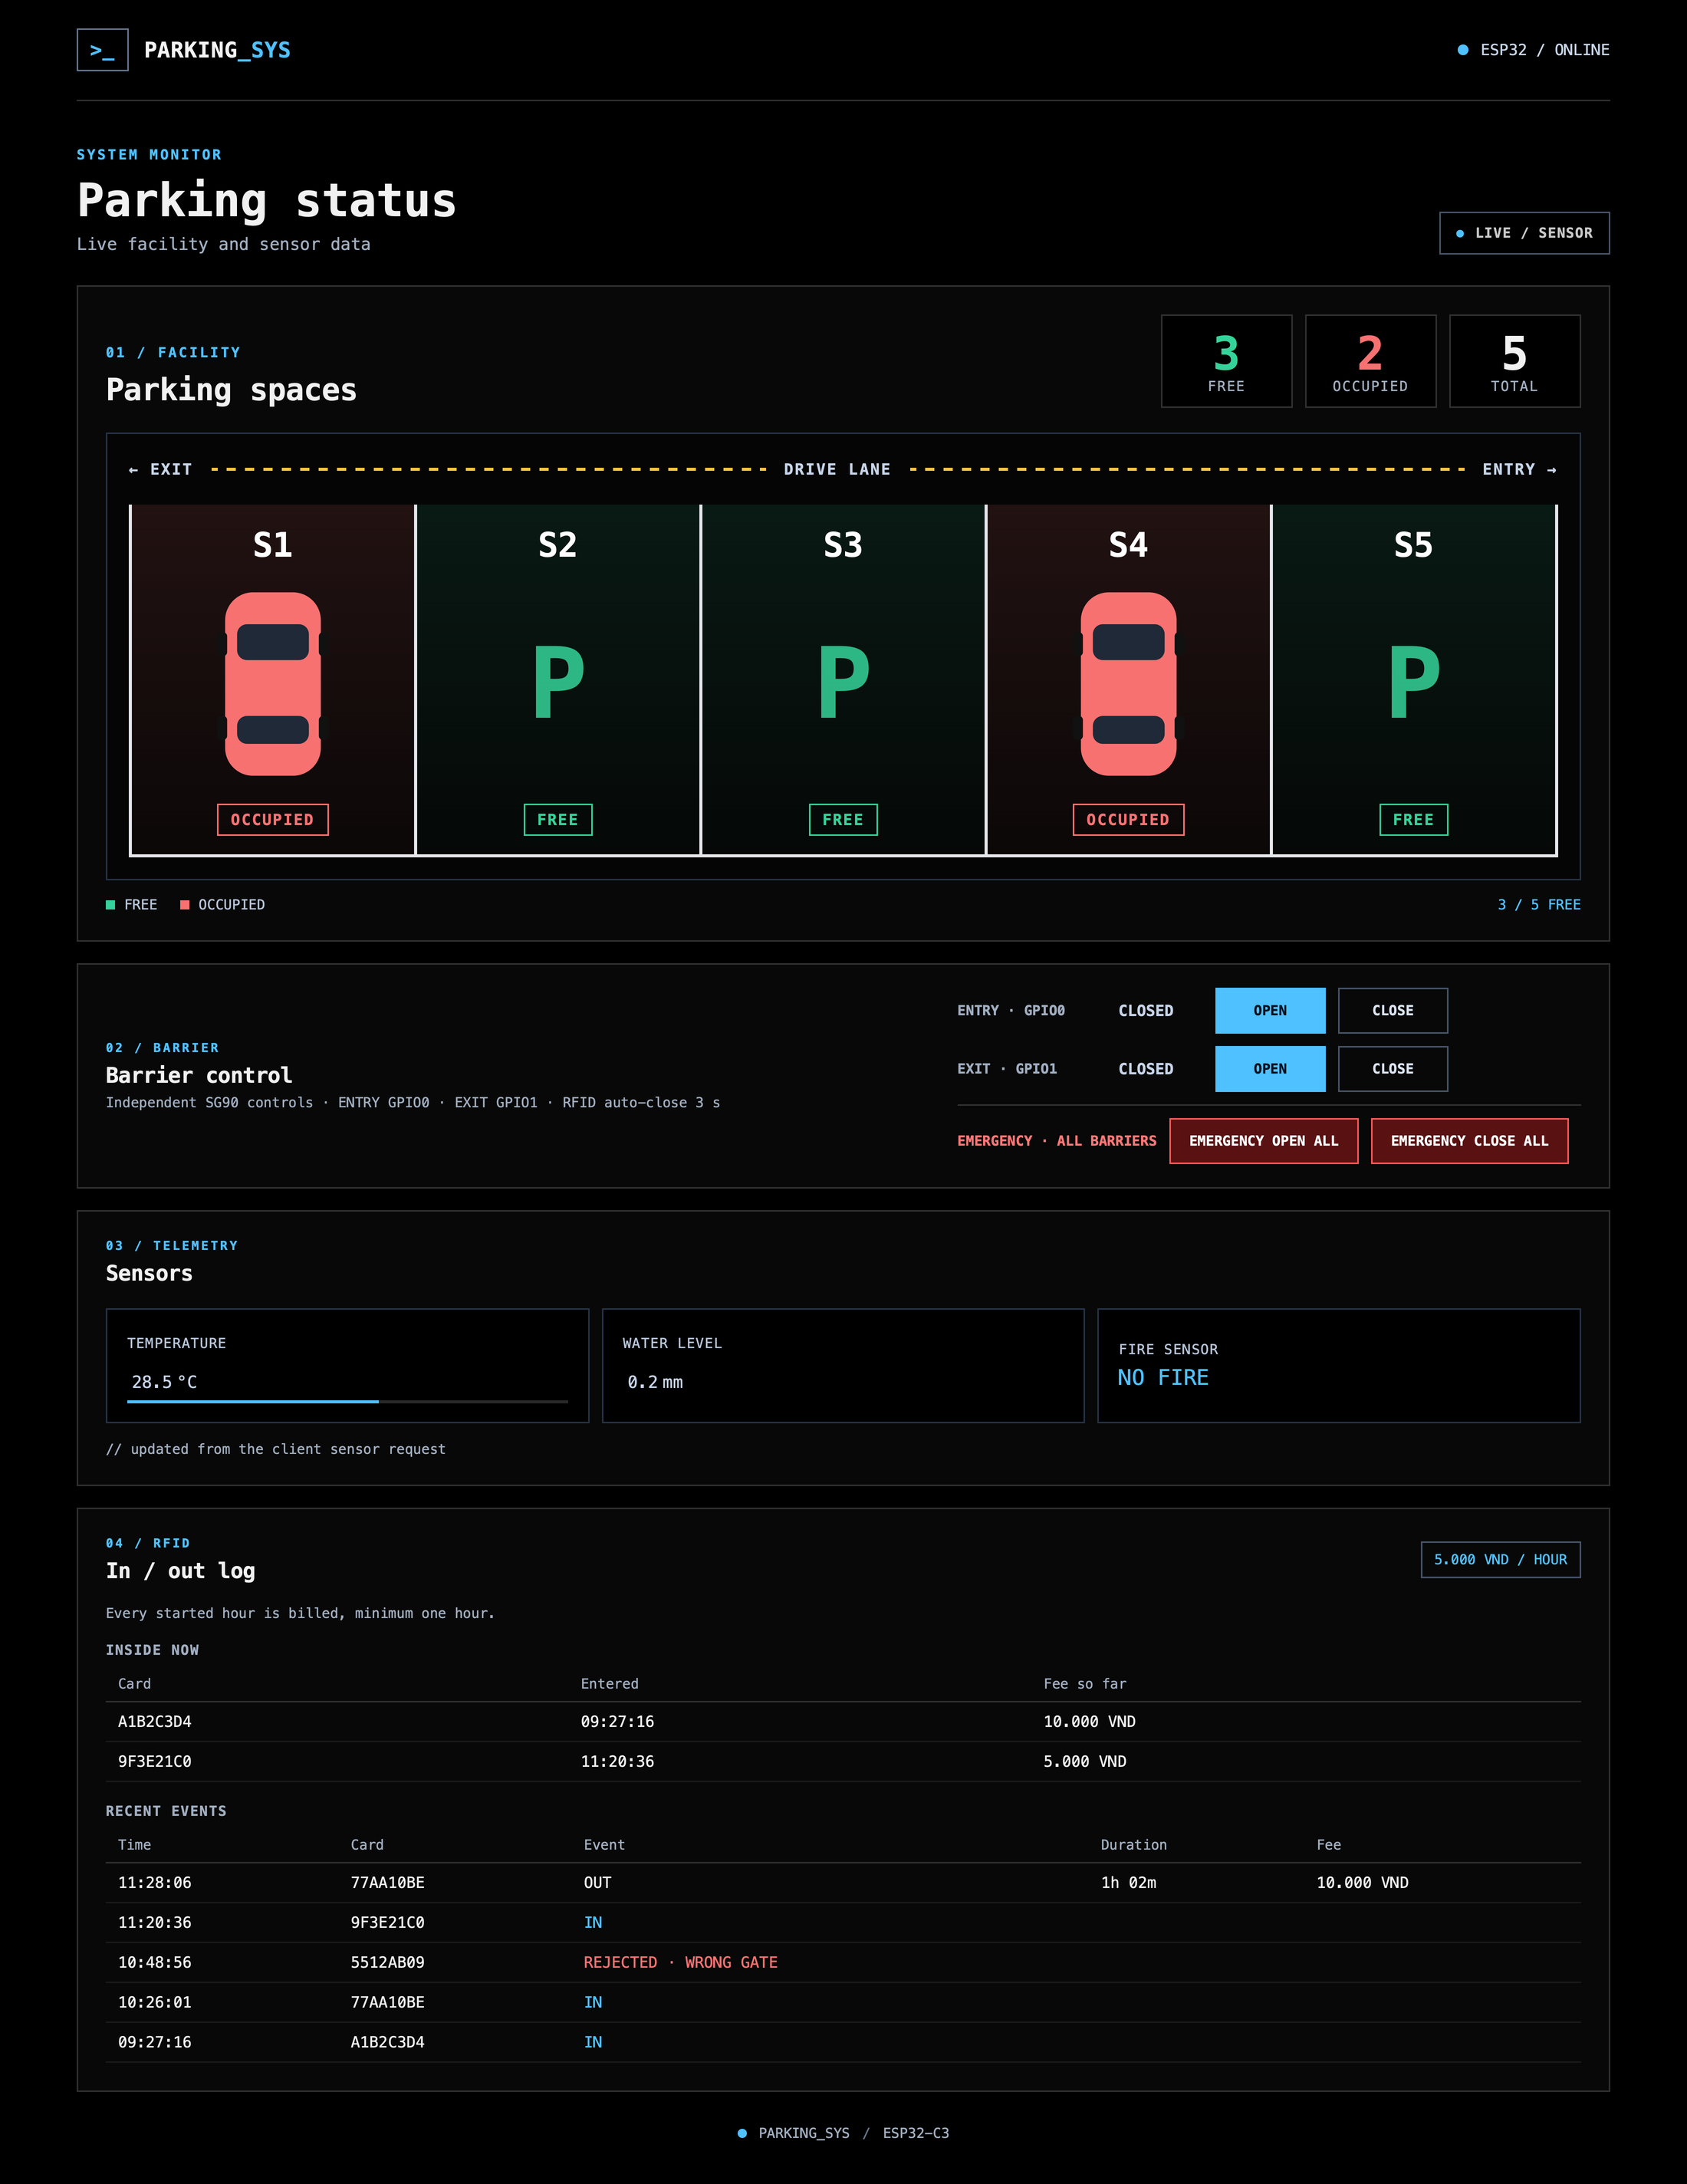
\includegraphics[width=0.86\linewidth]{dashboard.png}
\caption{Trang web giám sát tại \code{http://parking.local} (dữ liệu mẫu)}\label{fig:dashboard}
\end{figure}

\subsection{Các màn hình TFT}
\begin{figure}[H]
\centering
\setlength{\tabcolsep}{3pt}
\begin{tabular}{ccc}
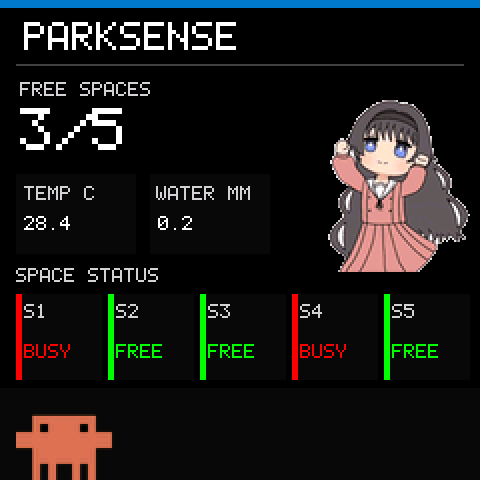
\includegraphics[width=0.3\linewidth]{photos/tft_main.png} &
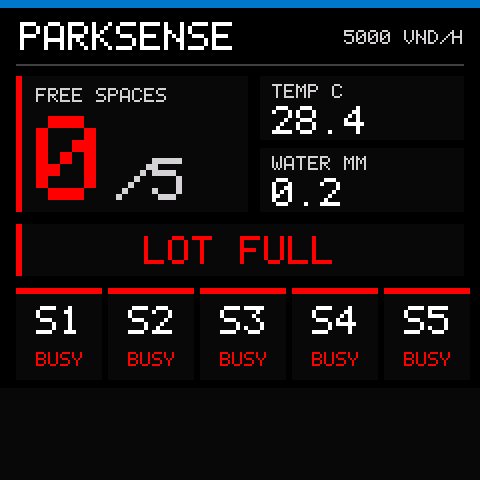
\includegraphics[width=0.3\linewidth]{photos/tft_full.png} &
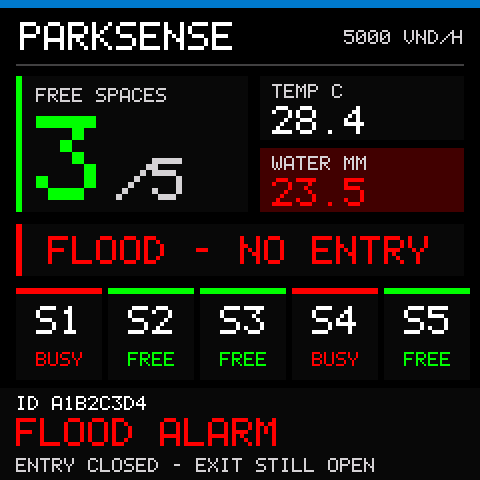
\includegraphics[width=0.3\linewidth]{photos/tft_flood.png} \\
\footnotesize (a) Bình thường & \footnotesize (b) Bãi đầy & \footnotesize (c) Ngập, quẹt vào bị từ chối \\[4pt]
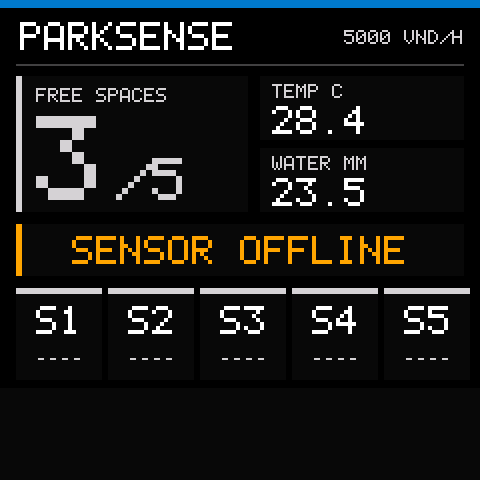
\includegraphics[width=0.3\linewidth]{photos/tft_offline.png} &
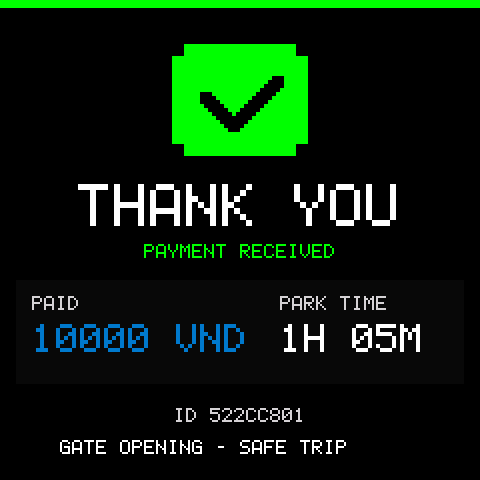
\includegraphics[width=0.3\linewidth]{photos/tft_thanks.png} &
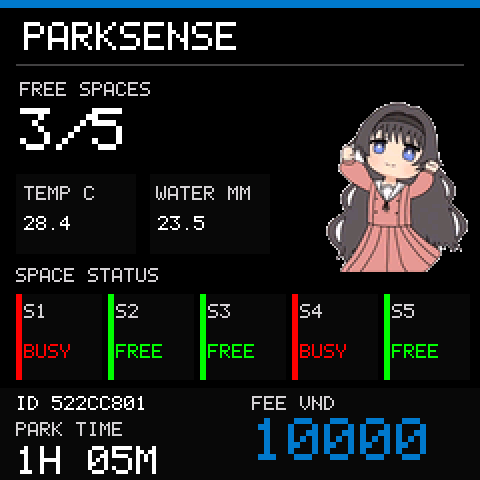
\includegraphics[width=0.3\linewidth]{photos/tft_receipt.png} \\
\footnotesize (d) Cảm biến mất kết nối & \footnotesize (e) Cảm ơn sau khi trả tiền & \footnotesize (f) Hóa đơn ở chân màn hình \\
\end{tabular}
\caption{Các màn hình TFT $240\times240$, kết xuất từ chính mã \file{lcd\_display.c} biên dịch trên máy tính}\label{fig:tft}
\end{figure}
Trên màn hình bình thường: hàng trên là số chỗ trống, hai ô nhiệt độ và mực nước (ô nước chuyển
đỏ khi ngập), ảnh động $96\times96$ ở góc phải; nhãn \code{FLOOD-NO ENTRY} hoặc \code{SENSOR OFFLINE}
hiện ở góc trên; hàng giữa là 5 ô S1–S5 với vạch xanh (trống)/đỏ (có xe); vùng chân dùng cho ảnh
động nhỏ, hóa đơn hoặc thông báo. Khi một lượt trả tiền hoàn tất (SePay hoặc
\emph{Confirm paid}), màn hình \code{THANK YOU} hiện 5\,s trong lúc thanh chắn mở, sau đó hóa đơn
vẫn ở chân màn hình thêm khoảng một phút.

\begin{figure}[H]
\centering
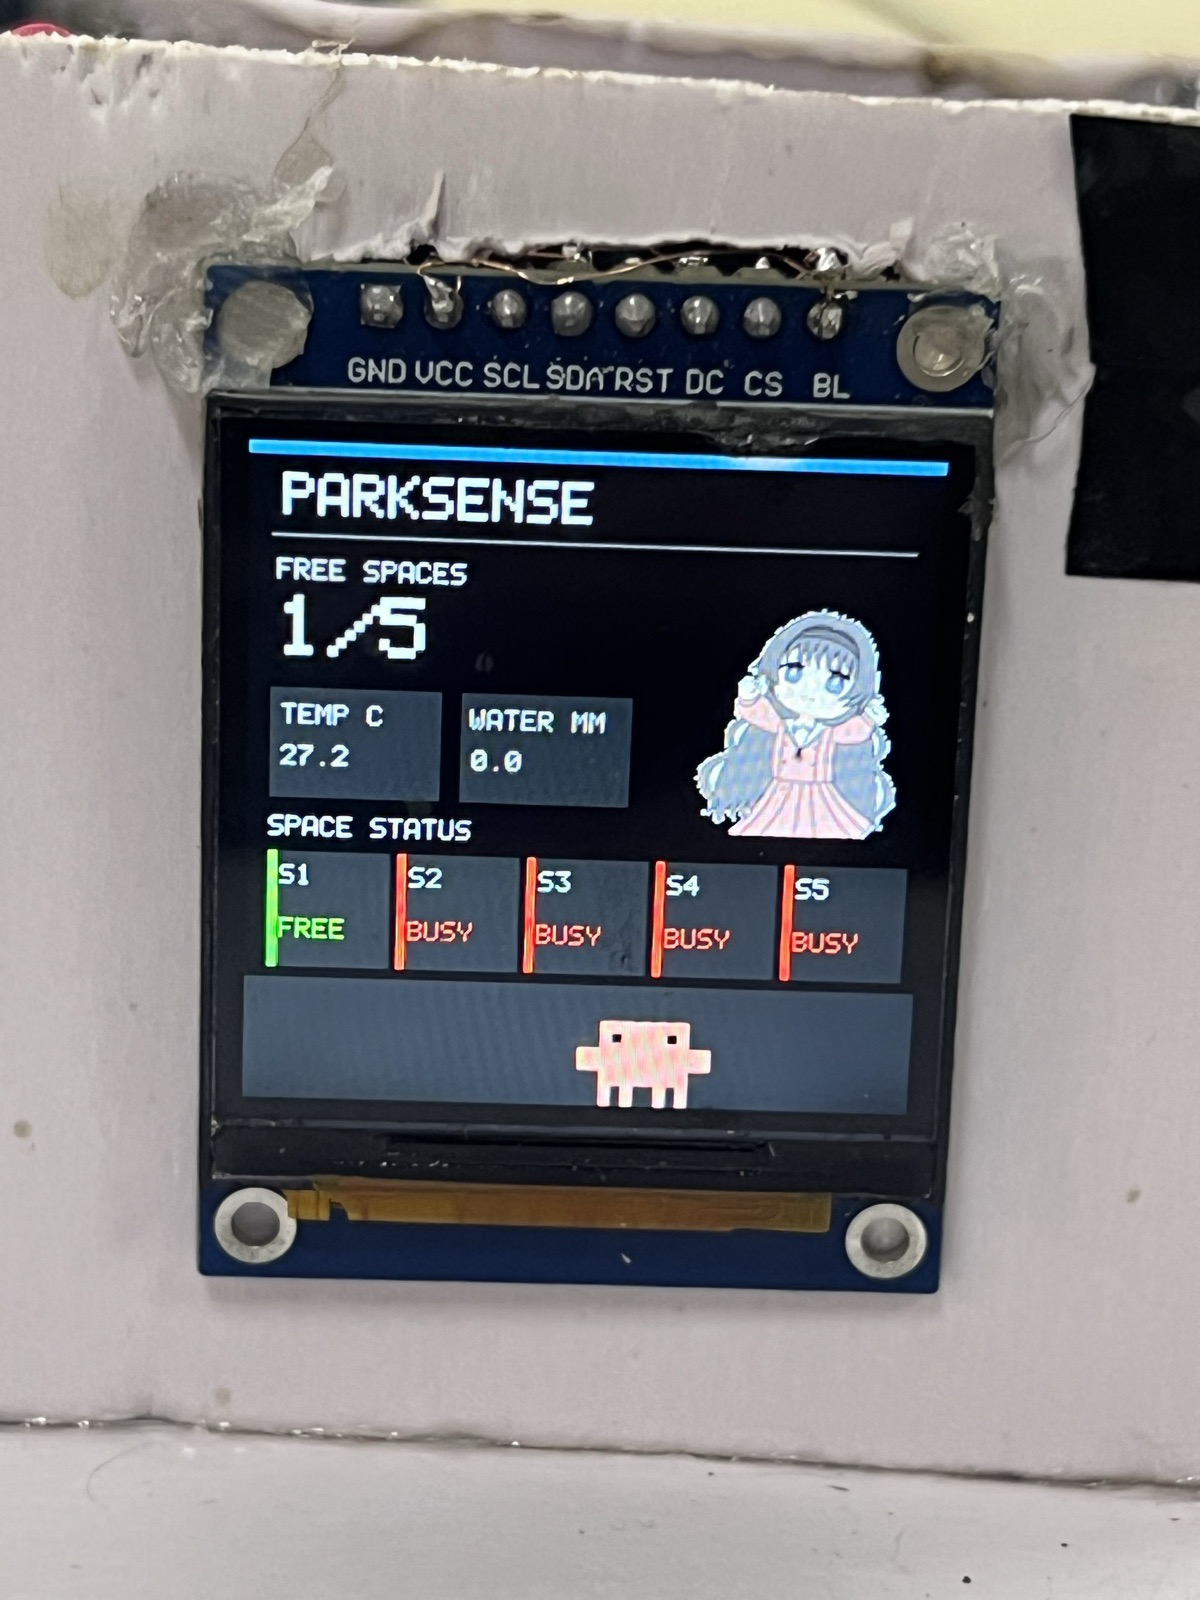
\includegraphics[width=0.42\linewidth]{photos/tft_live.jpg}
\caption{Màn hình TFT thật trên mô hình khi 4 ô có xe: \code{FREE SPACES 1/5}, S1 trống (xanh), S2–S5 có xe (đỏ), nhiệt độ 27,2\,°C, mực nước 0,0\,mm}\label{fig:tft-live}
\end{figure}

\subsection{Kịch bản demo}
\begin{enumerate}
\item Bật máy chủ, RFID Client, Sensor Client (thứ tự bất kỳ); điện thoại ở cùng mạng Wi-Fi chung mở \code{http://parking.local}.
\item Đặt xe mô hình vào ô S2: ô S2 trên TFT chuyển đỏ ngay, trên web hiện hình xe trong $\le$ 1\,s.
\item Quẹt thẻ ở cổng vào: thanh chắn vào mở rồi tự đóng sau 3\,s; web có dòng \code{IN}.
\item Quẹt lại thẻ đó ở cổng vào: màn hình báo \code{WRONG GATE – ALREADY INSIDE - USE EXIT GATE}.
\item Quẹt thẻ ở cổng ra: TFT hiện mã VietQR; quét bằng ứng dụng ngân hàng và chuyển khoản; vài giây sau hóa đơn hiện trên TFT, thanh chắn ra mở; web có dòng \code{OUT} kèm phí.
\item Đưa bật lửa gần cảm biến lửa: còi kêu, màn hình DANGER, hai thanh chắn mở và không đóng được từ web.
\item Tắt lửa: còi tắt, thanh chắn đóng, màn hình trở lại bình thường.
\end{enumerate}
\section{Đánh giá các chức năng đã hoàn thiện}
Nhóm đã xây dựng hoàn chỉnh một hệ thống bãi đỗ xe thông minh quy mô mô hình gồm ba
vi điều khiển, cùng kết nối vào mạng Wi-Fi chung của nhóm:
\begin{itemize}
  \item \textbf{10 use case} (Mục~\ref{chap:usecase}) đều được hiện thực: theo dõi chỗ
        trống tại bãi và trên web, gửi/lấy xe bằng RFID kèm tính phí, từ chối quẹt sai
        cổng hoặc bãi đầy, cảnh báo cháy và mở đường sơ tán, giám sát nước và nhiệt độ,
        điều khiển thanh chắn thủ công, nhật ký vào/ra kèm phí.
  \item \textbf{Thanh toán VietQR}: cổng ra hiển thị mã VietQR (BIDV) sinh ngay trên chip,
        máy chủ hỏi SePay mỗi 3\,s và tự mở thanh chắn khi nhận được chuyển khoản đúng mã
        và đủ tiền; khi không có Internet hoặc trả tiền mặt, người vận hành xác nhận trên
        trang web.
  \item \textbf{Kiến trúc} phân lớp rõ ràng, không có phụ thuộc vòng; đa tác vụ với
        FreeRTOS và ba cơ chế đồng bộ dùng đúng chỗ; giao tiếp UDP nhẹ, tự phục hồi khi mất gói;
        tên \code{parking.local} luôn trỏ đúng IP; ba bo đều là trạm Wi-Fi nên bật theo
        thứ tự nào cũng được.
  \item \textbf{Hiệu năng}: màn hình phản ánh thay đổi trong khoảng 0,1\,s; thanh chắn mở
        khoảng 0,2\,s sau khi quẹt thẻ; firmware dùng 31\% RAM tĩnh, còn 15\% flash ứng dụng.
  \item \textbf{Chất lượng}: 429 phép kiểm thử tự động đều đạt, chạy cả mã nguồn hai
        client trên phần cứng giả lập.
  \item \textbf{Bền vững}: quẹt thẻ không bị mất (ACK và gửi lại), dữ liệu gửi xe giữ được qua mất điện, giờ thực không cần Internet.
  \item \textbf{Giám sát chủ động}: phát hiện Sensor Client mất kết nối sau 3\,s thay vì
        hiển thị dữ liệu cũ như dữ liệu thật; cảnh báo ngập có trễ, tự chặn xe vào; thống kê
        doanh thu, lượt vào/ra theo ngày và 7 ngày.
  \item \textbf{Mô hình thực tế} hoàn chỉnh (Hình~\ref{fig:model}): 5 ô có cảm biến, 2 cổng
        servo, hộp điều khiển trung tâm có màn hình, nguồn có bảo vệ ngược cực.
\end{itemize}

Qua đề tài, nhóm đã vận dụng các kiến thức trọng tâm của môn lập trình nhúng: hệ điều
hành thời gian thực, đồng bộ tác vụ, PWM và SPI có DMA, ADC và lọc nhiễu tín hiệu số,
lập trình socket, quản lý bộ nhớ hạn chế, xử lý dữ liệu không tin cậy, và kiểm thử
phần mềm nhúng không cần phần cứng.

\section{Các hạn chế đã được khắc phục}
Bản thiết kế đầu tiên có năm hạn chế. Bốn hạn chế đã được khắc phục hoàn toàn, hạn
chế về bảo mật được khắc phục ở phía trang web và mật khẩu (bản tin UDP chủ đích không
ký, xem mục~\ref{sec:conlai}); tất cả được
kiểm chứng bằng kiểm thử tự động (Bảng~\ref{tab:unittests}) và kịch bản phần cứng
S15–S21 (Bảng~\ref{tab:systest}):

\begin{longtable}{@{}p{3.2cm}p{6.6cm}p{4.6cm}@{}}
\caption{Hạn chế ban đầu và giải pháp đã hiện thực}\label{tab:fixed}\\
\toprule \textbf{Hạn chế} & \textbf{Giải pháp} & \textbf{Kiểm chứng} \\ \midrule \endfirsthead
\toprule \textbf{Hạn chế} & \textbf{Giải pháp} & \textbf{Kiểm chứng} \\ \midrule \endhead
Bản tin UDP và API không có xác thực; mật khẩu cố định trong mã nguồn &
Lệnh POST cần mã PIN quản trị; mật khẩu Wi-Fi và mã PIN chuyển ra \file{sdkconfig}
(menuconfig) và \file{secrets.h}, không còn trong Git &
S19 \\ \midrule
Sự kiện quẹt thẻ có thể mất &
Máy chủ trả ACK; RFID Client gửi lại sau 300\,ms, tối đa 6 lần; máy chủ nhận ra
bản gửi lại qua \code{seq} nên không mở cổng hai lần &
\file{rfid\_client}: gửi lại, bỏ cuộc; \file{rfid\_session}: chống xử lý trùng; S16, S18 \\ \midrule
Phiên và nhật ký mất khi khởi động lại; thời gian tính từ lúc khởi động &
Toàn bộ trạng thái (\code{rfid\_store\_t}) lưu NVS sau mỗi lần quẹt và mỗi 5 phút, khôi
phục khi khởi động; trình duyệt của người vận hành gửi giờ Unix
(\code{POST /api/time}), máy chủ dời các mốc cũ theo và bù thời gian mất điện &
\file{rfid\_session}: lưu/khôi phục, đặt giờ; S17 \\ \midrule
Nhiệt độ chỉ cập nhật khi có xe quẹt thẻ &
RFID Client gửi bản tin \code{climate} mỗi 5\,s, độc lập với quẹt thẻ &
\file{rfid\_client}, \file{json\_parsers}; S21 \\ \midrule
Số phiên RFID và cảm biến IR chưa được đối chiếu &
Máy chủ từ chối thẻ mới khi IR báo đủ 5 ô có xe; trang web cảnh báo \code{CHECK THE LOT}
khi số thẻ trong bãi lệch số ô có xe quá 15\,s; số xe nhiều hơn số thẻ quá 15\,s thì còi kêu ngắt quãng và TFT hiện \code{CAR W/O CARD} &
\file{rfid\_session}: đối chiếu IR; S20 \\
\bottomrule
\end{longtable}


\section{Hạn chế còn tồn tại, nguyên nhân và cách khắc phục}\label{sec:conlai}
Các điểm dưới đây là đánh đổi có chủ đích ở quy mô mô hình, đã được ghi rõ trong mã nguồn
và hướng dẫn:
\begin{longtable}{@{}>{\raggedright\arraybackslash}p{3.8cm}>{\raggedright\arraybackslash}p{5.1cm}>{\raggedright\arraybackslash}p{5.3cm}@{}}
\caption{Hạn chế còn tồn tại}\label{tab:conlai}\\
\toprule \textbf{Hạn chế} & \textbf{Nguyên nhân} & \textbf{Cách khắc phục} \\ \midrule \endfirsthead
\toprule \textbf{Hạn chế} & \textbf{Nguyên nhân} & \textbf{Cách khắc phục} \\ \midrule \endhead
Trang web dùng HTTP, người cùng mạng có thể nghe được mã PIN & HTTPS cần chứng chỉ và thêm $\approx$ 40\,KB RAM cho TLS phía máy chủ & Bật HTTPS cho trang quản trị khi dùng chip nhiều RAM hơn (ESP32-S3 có PSRAM) \\
Bản tin UDP không được ký: thiết bị trong mạng có thể gửi thẻ giả, báo cháy giả & Chọn giao thức đơn giản, dễ gỡ lỗi trên mạng Wi-Fi riêng có WPA2 & Ký bản tin bằng HMAC kèm số thứ tự chống phát lại \\
Phụ thuộc router Wi-Fi chung; router bật cô lập thiết bị sẽ chặn broadcast & Ba bo giao tiếp qua điểm phát chung & Dùng router riêng cho bãi, tắt cô lập thiết bị; hoặc ESP-NOW giữa các bo \\
Token SePay có toàn quyền đọc giao dịch và nằm trong flash máy chủ & SePay không giới hạn quyền token; máy chủ phải tự gọi API & Mã hóa flash (flash encryption) hoặc chuyển việc gọi SePay sang một máy chủ trung gian dùng webhook \\
Mỗi lúc chỉ một xe thanh toán ở cổng ra & Một cổng ra, một màn hình QR; ví như MoMo bỏ nội dung chuyển khoản nên phải đối chiếu theo số tiền & Mỗi lượt một tài khoản ảo (VA) riêng theo đơn hàng \\
Ứng dụng ngân hàng có thể cho sửa số tiền; chuyển sai thì cổng không mở và tiền không được hoàn tự động & VietQR chỉ điền sẵn số tiền, việc khóa ô nhập do từng ứng dụng quyết định; máy chủ chỉ đọc được giao dịch & Thêm quy trình hoàn tiền của người vận hành, hoặc cổng thanh toán có hoàn tiền qua API \\
Xóa xe trên trang web không để lại dấu vết trong nhật ký; ai có PIN đều có thể cho xe ra mà không tính phí & Nút xóa chỉ dùng để sửa danh sách sai & Ghi một sự kiện \code{DELETED} vào nhật ký \\
Còi cảnh báo xe không thẻ không tắt được bằng tay; cảm biến IR bị che hoặc hỏng làm còi kêu mãi & Chưa có nút tắt còi; còi chỉ dừng khi hai số khớp hoặc cảm biến mất kết nối & Thêm nút tắt còi trên trang web \\
Chưa có trình duyệt nào gửi giờ sau mất điện thì thời gian mất điện chưa được tính & Máy chủ không có đồng hồ thời gian thực & Thêm module RTC DS3231 hoặc lấy giờ qua SNTP khi có Internet \\
\bottomrule
\end{longtable}

